\section{Results and Discussion}

\subsection{Parameter Tuning}

\begin{figure}[!htbp]
\begin{center}
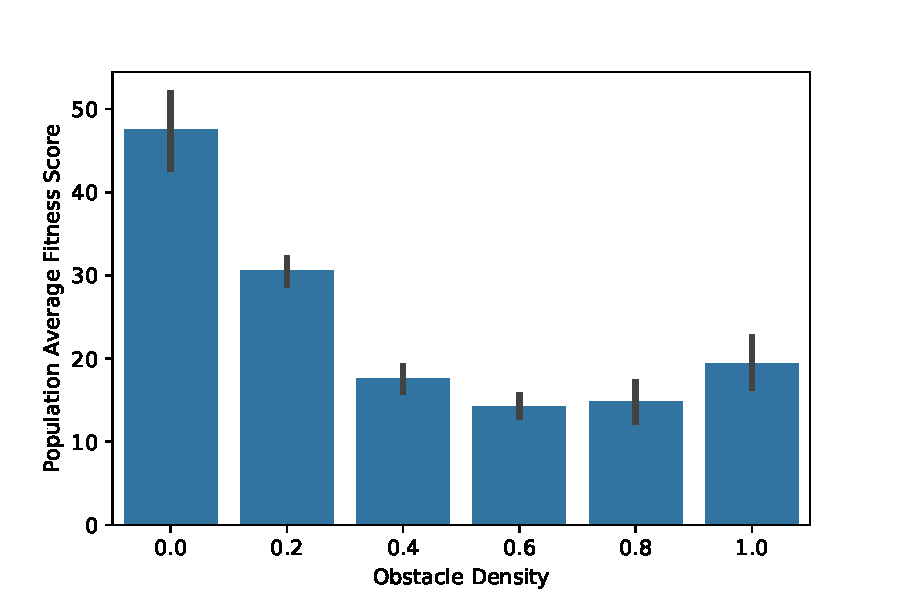
\includegraphics[width=\textwidth]{img/obstacle_density_average_fitness.pdf}
\caption{
Caption TODO
}
\label{fig:obstacle_density_average_fitness}
\end{center}
\end{figure}

\begin{figure}[!htbp]
\begin{center}
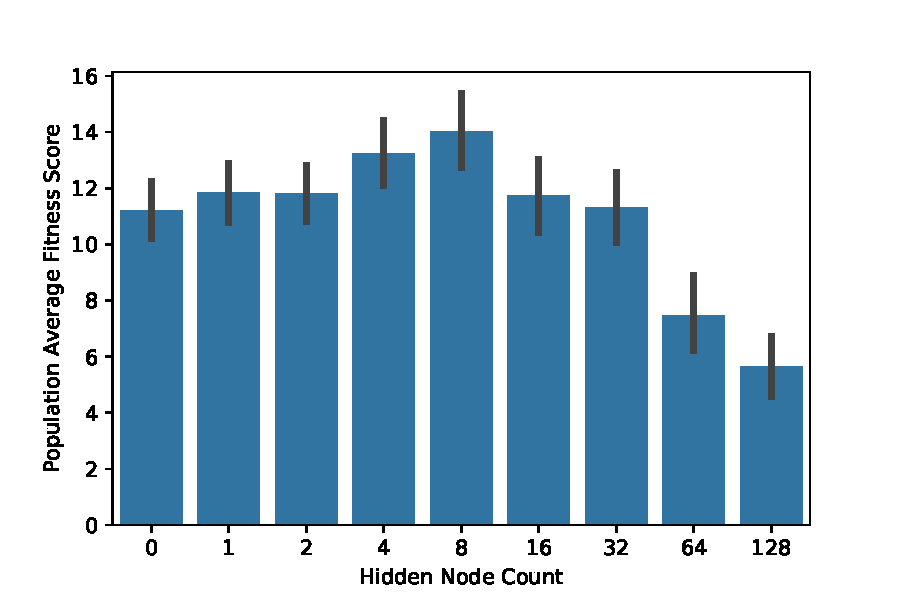
\includegraphics[width=\textwidth]{img/hidden_node_count_average_fitness.pdf}
\caption{
Population mean foraging performance at 20,000 generations in evolutionary runs with stigmergic cues disabled over different Markov brain hidden node counts.
Error bars indicate 95\% confidence intervals.
}
\label{fig:hidden_node_count_average_fitness}
\end{center}
\end{figure}


First, we investigated the nature of our foraging task by analyzing the relationship between foraging performance and obstacle density.
We ran 166 replicate 20,000 generation evolutionary trials, varying obstacle density from a completely empty space (0.0) to a full depth-first search maze space (1.0).
For these experiments, we used an intermediate stigmergy evaporation delay of 10 updates and Markov brains with 8 hidden nodes.
As would be expected, foraging performance was highest for low obstacle density;
population average foraging performance at obstacle density of 0.0 was significantly greater than that at 0.2 and both had significantly greater population average foraging performance than higher obstacle densities.
($p < 0.05$; independent t-test; Figure \ref{fig:obstacle_density_average_fitness}).
Interestingly, foraging performance was significantly greater at complete maze density (1.0) than at intermediate maze density (0.6) ($p < 0.05$; independent t-test; Figure \ref{fig:obstacle_density_average_fitness}).
Video playbacks of agent navigation behaviors at intermediate maze densities revealed that agents occasionally entered protracted navigational cycles, ``walking in circles'' around obstacles.
We believe that the increase of foraging performance at complete maze density might be due to the lack of available circuits for such navigational cycles in the complete depth-first search maze, preventing agents from becoming trapped in such quagmires.
We chose to run all subsequent experiments at an intermediate obstacle density of 0.5, which we believe most closely resembles the biological ant foraging scenario.

In order to ensure that stigmergic and non-stigmergic foraging strategies were on as even footing as possible, we investigated how the number of Markov brain hidden nodes affected evolved foraging performance with stigmergic navigation cues disabled (i.e., with knocked-out stigmergy read capacity).
We performed 20,000 generation evolutionary runs over a range of Markov brain hidden node counts with stigmergic navigational cues disabled.
Each treatment was replicated in 111 independent runs.
Figure \ref{fig:hidden_node_count_average_fitness} shows the relationship between Markov brain hidden node count and foraging task performance observed in these experiments.
Unsurprisingly, performance was maximized at an intermediate Markov brain hidden node count, which provides a balance between enabling sophisticated behaviors and inducing evolvability issues related to vanishing probability of useful connectivity establishment due to excess nodes.
To maximize the potential performance of non-stigmergic foraging strategies relative to stigmergic strategies, we chose to run all subsequent experiments with eight Markov brain hidden nodes.

\subsection{Pheromone Evaporation Rate and Foraging Task Performance}
\begin{figure}[!htbp]
\begin{center}
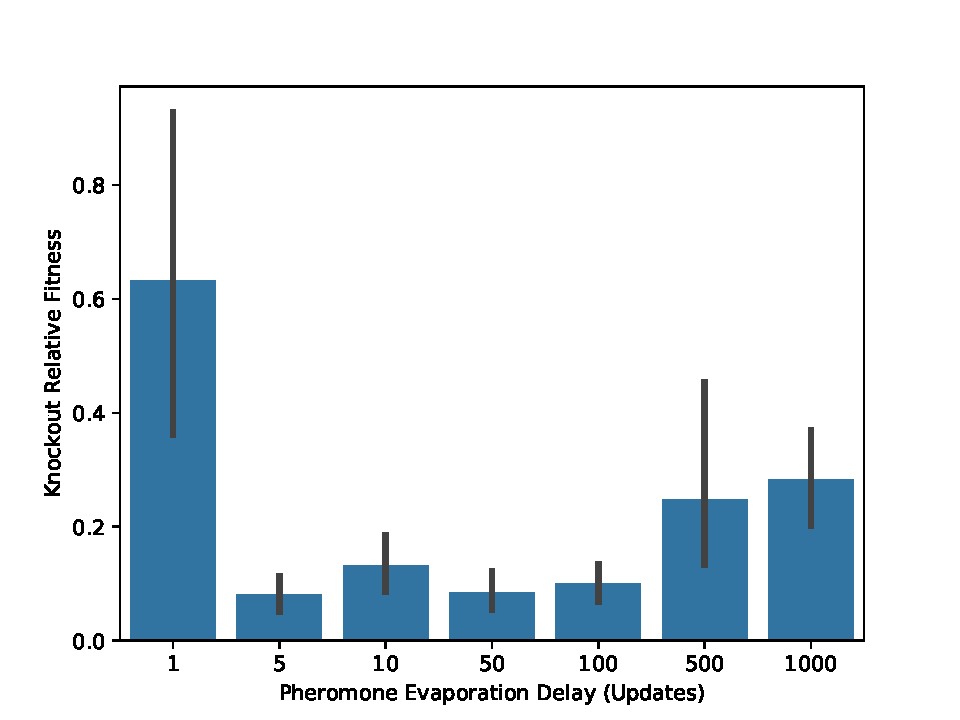
\includegraphics[width=\textwidth]{img/knockout_rel_fit_stig_delay.pdf}
\caption{
Caption TODO
}
\label{fig:knockout_rel_fit_stig_delay}
\end{center}
\end{figure}

\begin{figure}[!htbp]
\begin{center}
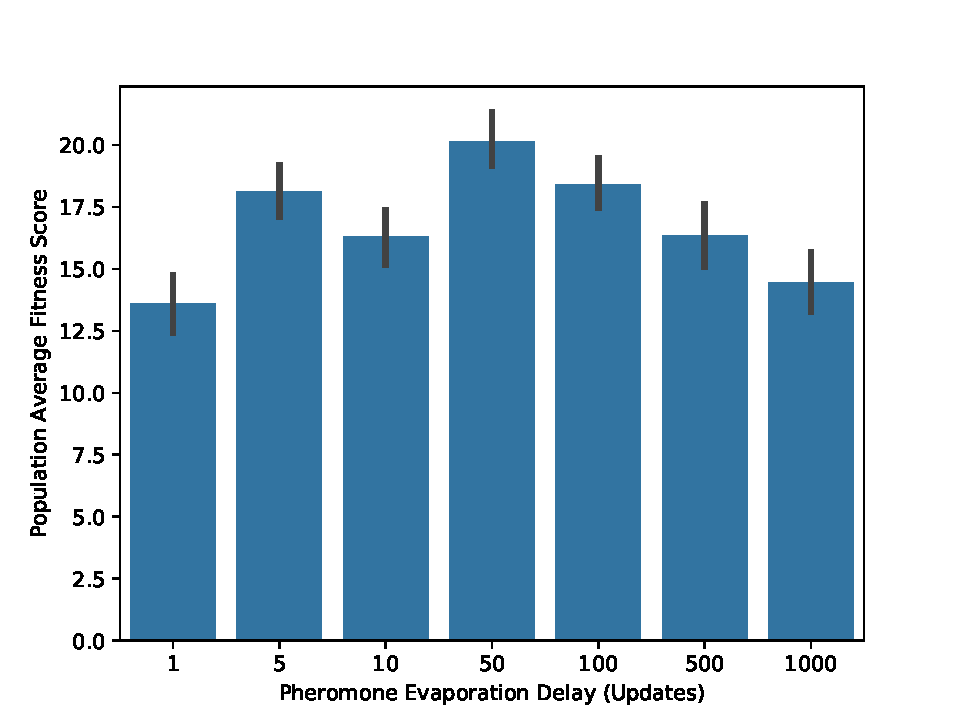
\includegraphics[width=\textwidth]{img/pheromone_evaporation_delay_average_fitness.pdf}
\caption{
Population average foraging performance at 20,000 generations in evolutionary runs with stigmergic cues disabled over different pheromone evaporation delays.
Error bars indicate 95\% confidence intervals.
}
\label{fig:pheromone_evaporation_delay_average_fitness}
\end{center}
\end{figure}


%\subsection{Pheromone Evaporation Rate and Food Permanence}
